\chapter{可见光多波段自适应通信系统硬件设计}
\section{引言}
我们在前面四章介绍了可见光通信的基本原理及关键技术,特别针对自适应传输这个核心重点研究了信道估计及比特功率分配算法,并且针对本课题对应的硬件平台的实际情况进行了必要的仿真,选出了合适的技术方案,如使用低复杂度的LS 算法进行信道估计、使用高精度的EVM方法进行信噪比估计、使用专为可见光通信设计的Improved-SBLA比特功率分配算法得到自适应参数。本章将对可见光通信的硬件系统做一个简要的介绍,还将概述自适应模块的逻辑设计。
\section{硬件平台概述}
本课题对应的硬件演示平台如图\ref{fig:Hardware_Structure}所示,该系统目前已经实现了“编译级”的自适应传输,所谓“编译级”就是代码支持通过改变调制参数然后需要再编译来实现调制的改变,而真正的自适应传输系统因为时间紧迫及反向链路方案尚未确定等因素没有完成。不过本系统已有了自适应传输的雏形了,只是信道估计、计算自适应参数、改变调制等需要离线进行,下面对该系统进行概述。
\begin{figure}[htbp]
\centering
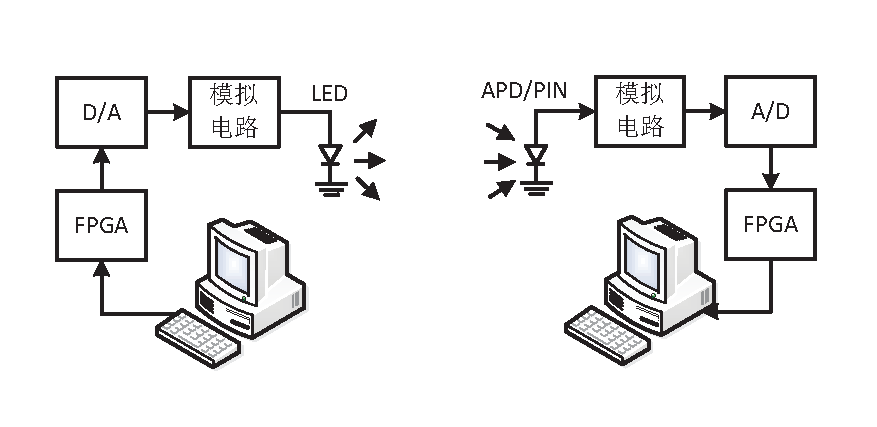
\includegraphics[width=0.8\textwidth]{figures/chapter-5/Hardware_Structure.eps}
\caption{可见光通信硬件平台示意图}
\label{fig:Hardware_Structure}
\end{figure}

首先信源比特通过以太网接口(UDP协议)按帧发送到用于基带处理的FPGA芯片(整个传输过程都是按帧进行的,并且用于同步和信道估计的ZC序列符号只在帧头处放置,整个帧中所有的OFDM符号都使用这个ZC序列估计出来的信道参数解调),接着在FPGA中完成扰码、信道编码、调制和IFFT等数字处理过程,然后将时域数字信号输入到数字模拟变换器(Digital to Analogue Converter,DAC)变成模拟信号,最后该模拟信号加上偏置电流之后去驱动LED灯,整个发射过程完成。接收端通过PD 接收LED光信号,并将光信号强弱的变化转换成电信号的大小,然后将此模拟电信号送入模拟/数字变换器(Analog to Digital Converter,ADC)中抽样量化为数字信号,再送到接收端基带处理FPGA进行解调、解码和校验等操作,最后输出接收到的帧到接收端计算机。
\subsection{硬件型号及参数简介}
本系统中用于基带处理的FPGA芯片选择美国Xilinx公司生产的Virtex-6,具体型号为XC6VSX315T,基于40 nm工艺,具有高性能、接口丰富等多方面优点。该芯片内部包含49,200个片逻辑单位,每个片逻辑单元中有4个查找表(Look Up Table,LUT)和8个触发器;内置1,344个DSP48数值计算块,每个数值计算块中包含一个$25\times 18$bit 乘法器、一个加法器和一个累加器;同时还有最大存储容量为25,244 kb的嵌入式存储RAM;并且支持千兆网卡\cite{FPGAIntroduciton}。这些资源为我们下面的基带逻辑处理及复杂的LDPC解码运算提供了硬件基础。

DAC选用美国TI公司生成的八通道高速数模转换芯片,型号为DAC3484,其输入数值信号位宽为16 bit,最高支持1 GSps的采样率;ADC芯片同样使用TI公司产品,型号为DAC9643,该芯片支持最高达250 MHz的采样速率,量化精度为14比特。

发射端模拟电路主要包括三部分,功率放大器、直流偏置模块和LED灯。功率放大器选用美国Mini-Circuits公司的ZHL-3A中功率放大器,其3 dB 带宽范围是0.4 MHz ~150 MHz,功率增益25 dB,最大输出功率为 30 dBm;采用的直流偏置模块ZFBT-6GW+同样是Mini-Circuits公司产品,其3 dB带宽范围为0.1 MHz~6 GHz,支持最大偏置电流0.5 A。发光二极管选用美国硅谷光擎(LED Engin)生产的多色混光型发光二极管LED——LZC-03MA07,其发光光谱图如图\ref{fig:LED_LZ4_relativeSputrcalPower}所示。

接收端模拟电路主要由滤光片、光电二极管即放大器。本系统为可见光多波段通信系统,不同的色光用不同的滤波片,分别是蓝光滤光片DTB435、绿光滤光片DTB530、红光滤光片HB610。光电转换模块选用雪崩型光电二极管(APD),具体型号为C5331-11,生产商为日本滨松公司(Hamamatsu),其3 dB通带为4 KHz~100 MHz,感光区直径1 mm。 接收端低噪声放大器选用美国TI公司生成的OPA847,其带宽增益积为3.9 GHz,输入噪声为$0.85 nV/\sqrt{Hz}$
\subsection{发射端基带处理}
\begin{figure}[htbp]
\centering
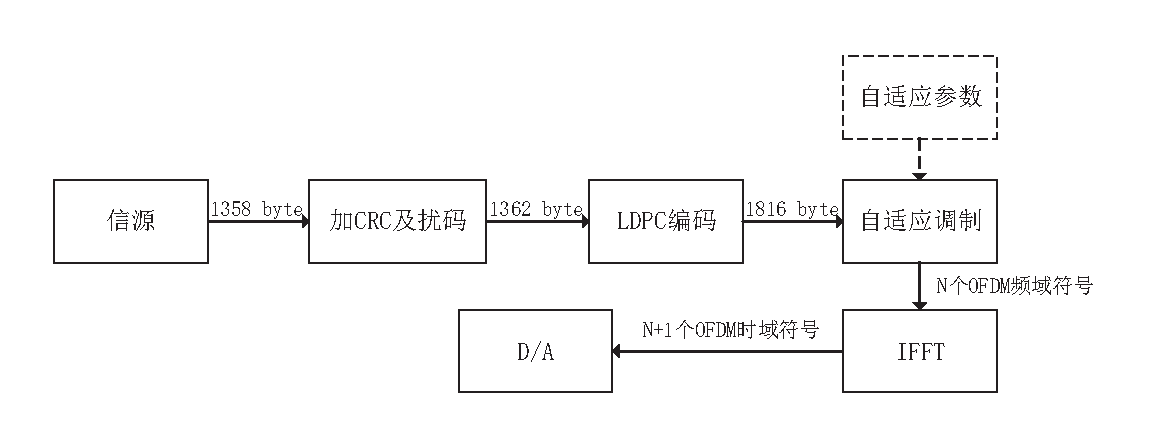
\includegraphics[width=0.9\textwidth]{figures/chapter-5/TransmitterSchematic.eps}
\caption{发射端基带处理原理框图}
\label{fig:TransmitterSchematic}
\end{figure}
发射端FPGA基带处理流程如图\ref{fig:TransmitterSchematic}所示,本演示系统信源帧长定为1358 byte (设置为该值主要是因为本系统主要以视频传输演示为主,而视频帧帧长就是1358 byte),为了系统设计简便起见,当通过以太网接口接到的帧不足1358 byte 时,会自动在后面补零再传输。

基带处理芯片接收到信源帧之后,第一步就是对其加循环冗余校验(Cyclic Redundancy Check,C RC),这里我们使用24 bit 的循环校验码,循环校验比特的生成模块其实就是一个由生成多项式决定的除法电路,输入数据就是被除数,而余数就是我们需要的校验比特,当然为了加快计算速度,本系统CRC使用8位并行计算方法,即不是想真的除法电路那样逐比特地输入,而是一次输入8 比特,整个运算速度提高了8倍。由于篇幅限制,在这里就不对CRC模块再进行过多的展开。得到24 bit(3 byte)校验位之后添加到原信源数据之后,又因为本系统使用的是输入为1362 byte 的低密度奇偶校验码(Low Density Parity Code,LDPC)作为信道编码,所以1358 byte数据帧加入3 byte 的校验码之后还要补零1 byte。为了防止过长的连0连1影响系统传输性能,所以还要把加了CRC及补零后的数据进行扰码再送入LDPC编码器。

信道编码是通过在发射数据中增加冗余以便在接收端可以进行信道解码纠错,本系统使用码率为3/4的LDPC码,输入数据长度为$1362\times 8$ bit,输出为14528 bit选择LDPC码的原因是其纠错性能佳,几乎适合所有信道,并且相对于Turbo码而言其解码器实现复杂度要低很多。这里使用的LDPC码的编码矩阵大小为$48\times 227$,所以输入数据位宽要为48 bit,而我们在CRC模块中输出数据位宽为8 bit,所以这里需要位宽变换,可以使用FPGA提供的RAM或先入先出队列(First In First Out,FIFO)数据结构来实现。编码之后的校验比特插在等间隔的插在信息数据中间,因为码率为3/4,每6字节信息数据后插入2个校验字节。

\begin{figure}[htbp]
\centering
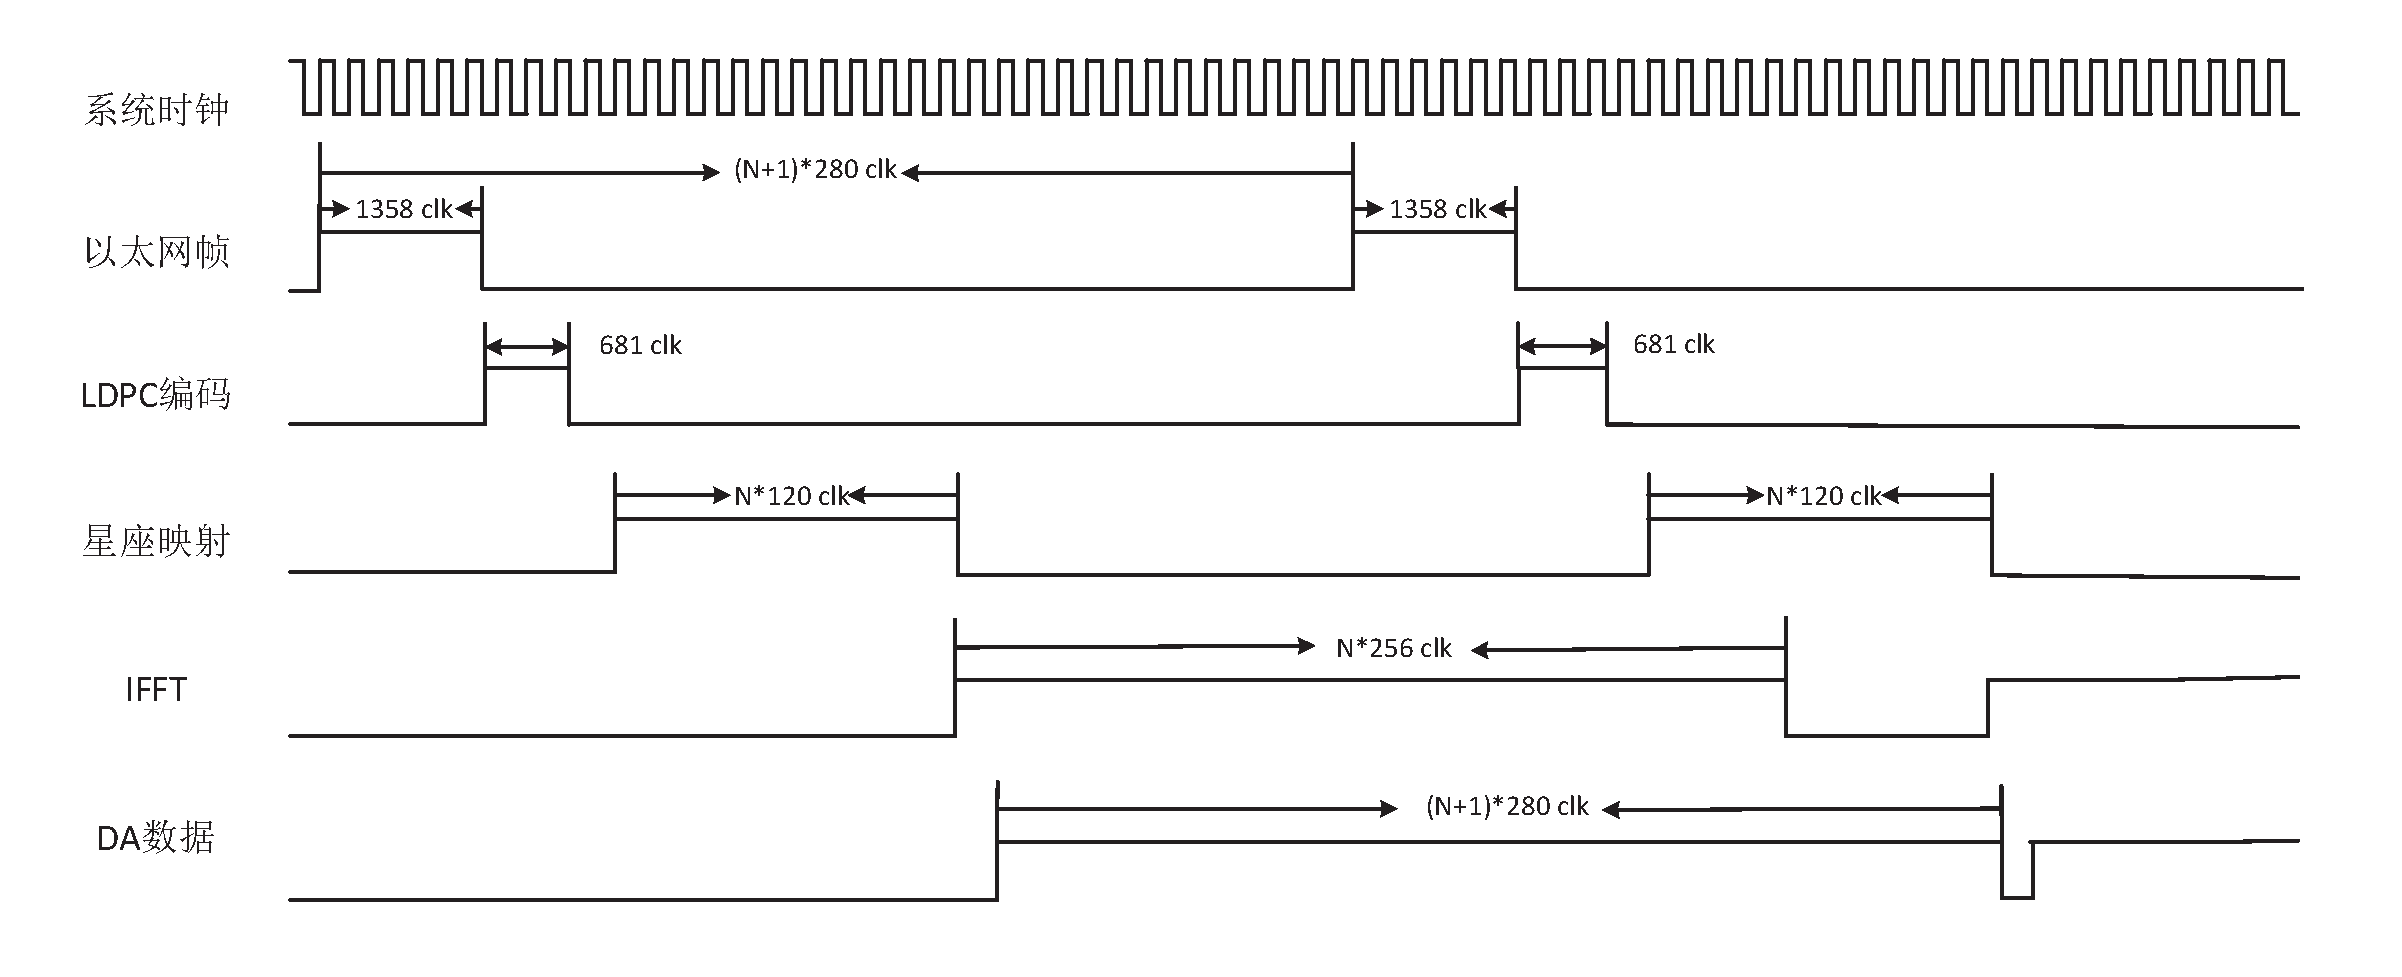
\includegraphics[width=0.9\textwidth]{figures/chapter-5/TimeSchemeTrans.eps}
\caption{发射端基带处理时序图}
\label{fig:TimeSchemeTrans}
\end{figure}
经过编码的帧数据长度变为1816 byte,送入自适应调制模块,其功能是将信息比特分配到OFDM各个子载波上,并映射到星座图中的点,输出OFDM符号频域数据,这部分属于自适应设计的核心部分,将在下一节详细介绍。

经自适应模块调制后得到N个OFDM符号,N的值也调制的选择有关,假设根据自适应参数每个OFDM符号传输R比特,则有N=$\lceil 14528/\text{R} \rceil$,其中$\lceil \cdot \rceil$表示向上取整运算。为了提高传输速率,要保证所有的操作在一个OFDM帧周期内完成,所以要将将已调制符号交替存入两个RAM中,进行乒乓操作,即如果自适应模块再往其中RAM中写数据,则IFFT模块应该在另一个RAM中读数据去进行IFFT运算,到下一帧时这两个RAM的角色交换。IFFT模块可以使用Xilinx 公司提供的IP核实现,并且可以通过设置自动添加添加循环前缀,非常方便。得到OFDM时域符号之后,在每帧的头部再加上ZC导频序列之后输入到DAC芯片输出,整个发射过程的时序安排如图\ref{fig:TimeSchemeTrans}所示。
\subsection{接收端基带处理}
\begin{figure}[htbp]
\centering
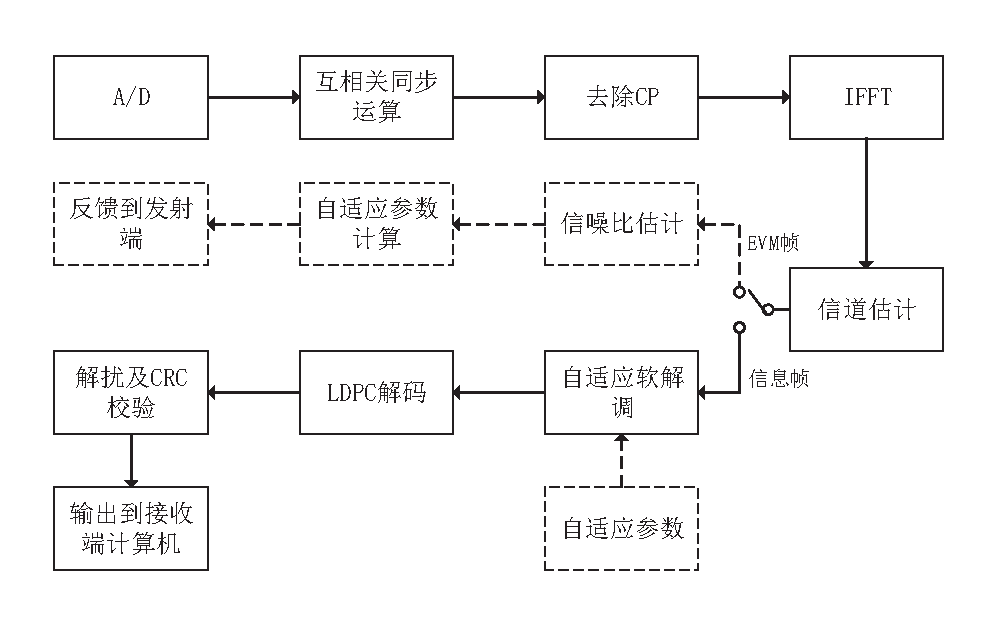
\includegraphics[width=0.9\textwidth]{figures/chapter-5/ReciverSchematic.eps}
\caption{接收端基带处理原理框图}
\label{fig:ReciverSchematic}
\end{figure}
接收端基带处理过程如图\ref{fig:ReciverSchematic}所示,模拟信号经过AD变化之后先与导频时域ZC 序列进行互相关同步运算,互相关结果的峰值所在位置就是导频的开始位置,在现实时为了避免找最大值这样复杂的运算,会通过另外一个模块估计接收信号的功率,从而得到一个互相关阀值,如果互相关结果大于这个阀值就可以认为是同步峰。使用这个特性就能把接收到的信号重新分成一个个OFDM符号,包含1个导频符号和N个信息符号。

因为要使用EVM方法进行信噪比估计,此时需要将用于EVM估计的前导序列放在信息符号发送,我们称这种帧为EVM帧。将这些时域OFDM符号去掉CP,再送入FFT模块,FFT模块输出频域OFDM符号,其中导频符号用于信道估计(使用LS算法),待得到信道估计之后,对信息符号进行单系数均衡,如果是数据帧则送入自适应软解调模块就行解调;如果是EVM帧怎送入信噪比估计模块估计SNR,之后再使用Improved-SBLA算法计算自适应参数,反馈到发射端,这部分也将在下一节展开。
\begin{figure}[htbp]
\centering
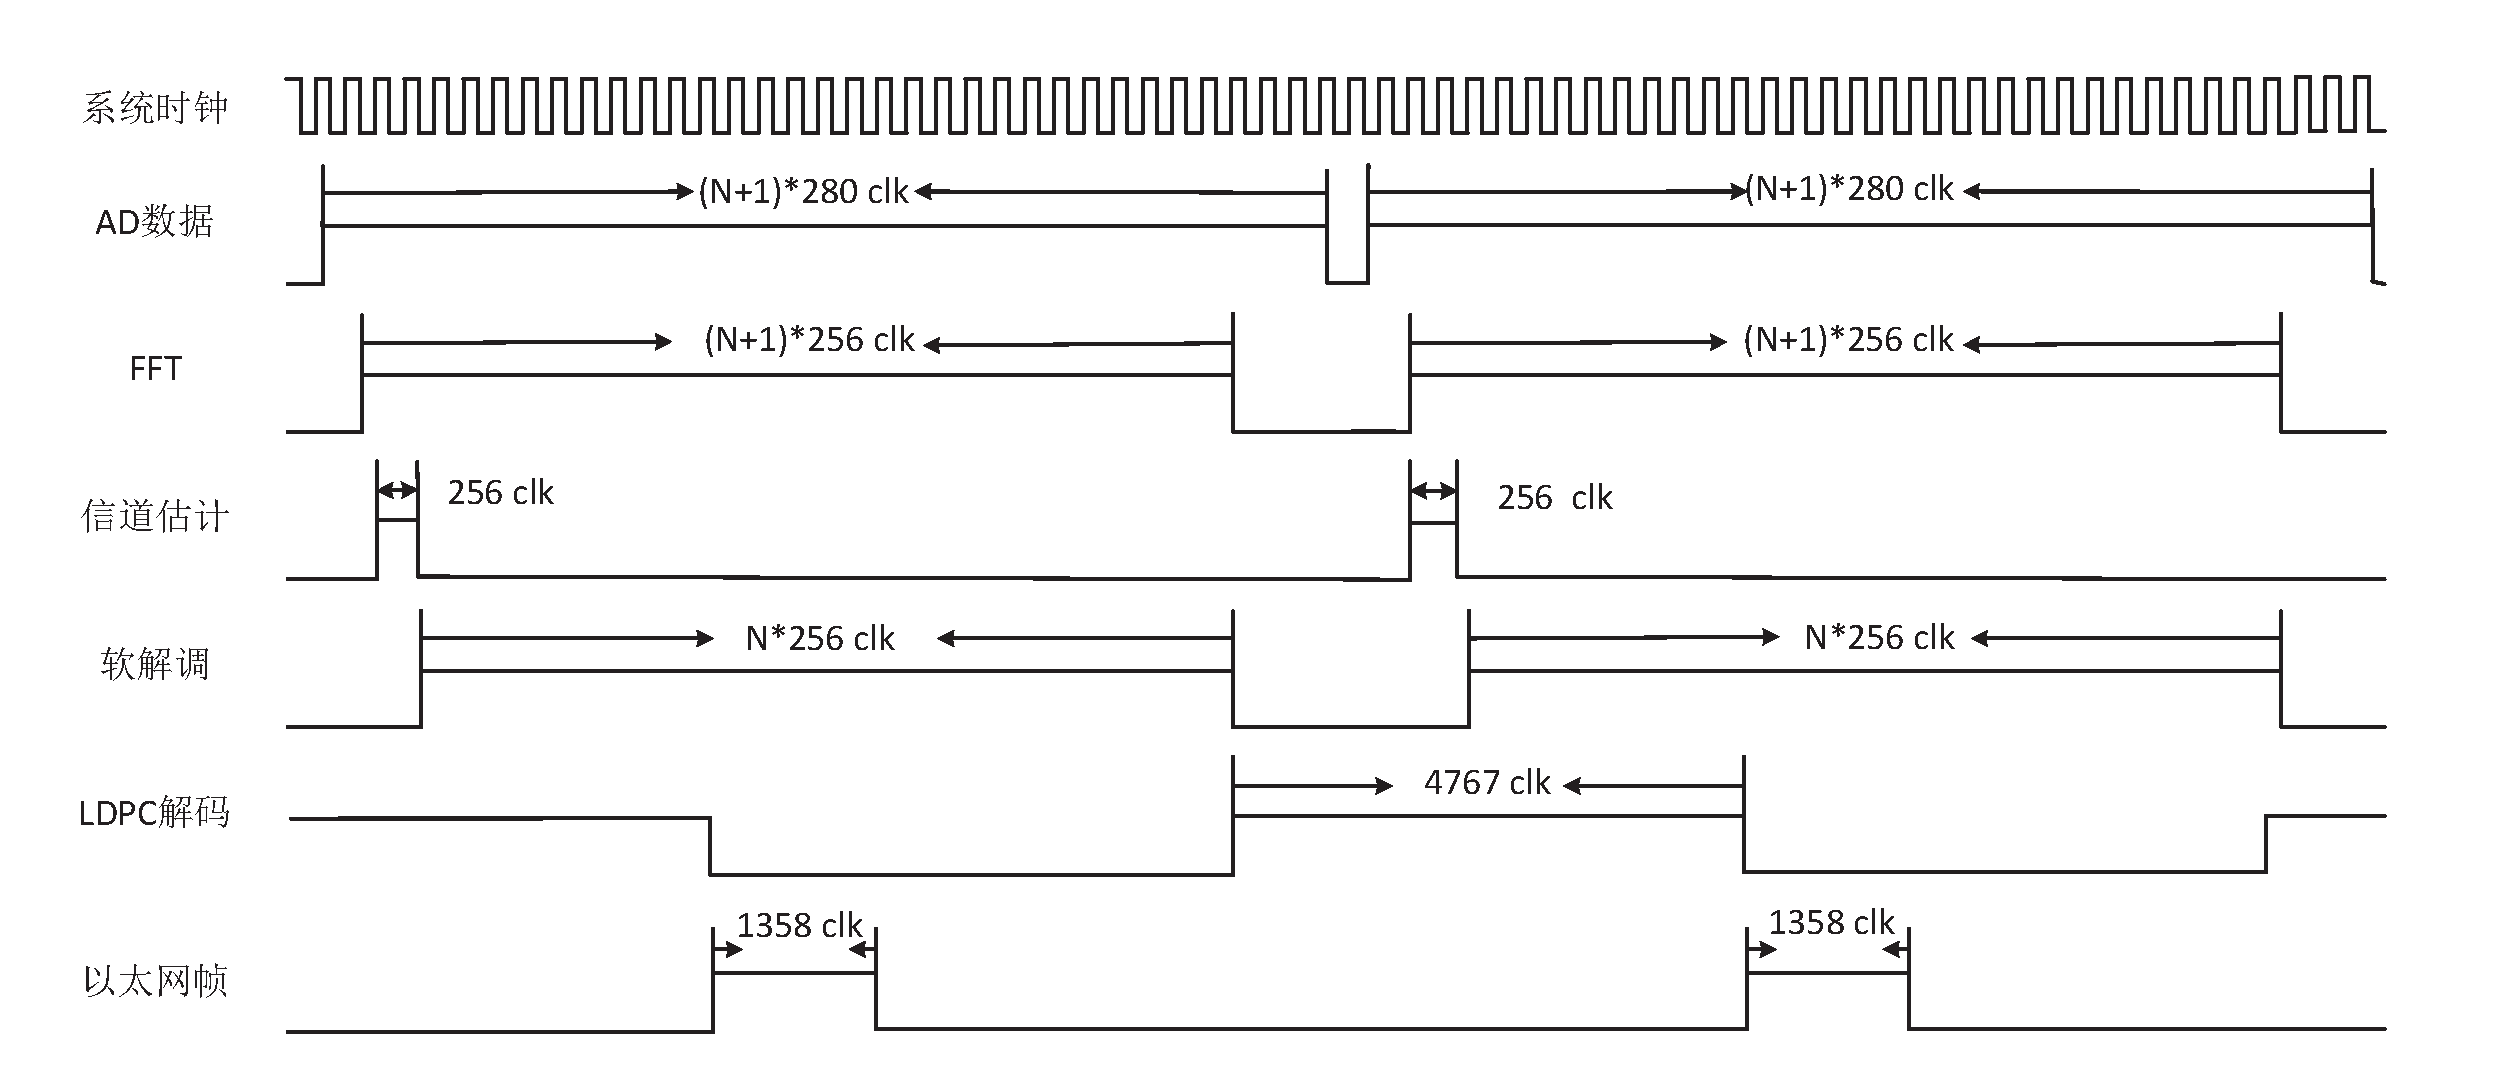
\includegraphics[width=0.9\textwidth]{figures/chapter-5/TimeSchemeRece.eps}
\caption{接收端基带处理时序图}
\label{fig:TransmitterSchematic}
\end{figure}

软解调得到的软件被送入LDPC码解码模块进行解码,软解调的输出位宽因调制阶数不同不同,如使用4QAM调制的子载波软解调输出位宽为16($8\times 2$)bit、16QAM为32 ($8\times 4$)bit、64QAM为48($8\times 6$)bit、256QAM对应为64($8\times 8$)bit,而解码器的输入位宽为$256=8\times 32$ bit,所以这里也存在数据位宽变换的问题,可以先将各阶调制得到的软量存在各自的RAM中,然后统一以64 bit位宽读出到一个FIFO中,再以256 bit位宽读出送入LDPC解码器解码。如接收端基带处理时序图\ref{fig:TransmitterSchematic}所示,解码过程所需要的时间也迭代次数成正比,具体为迭代次数加1再乘以227,本系统设置迭代次数为20,故整个解码过程为4767 clk。 解码器输出位宽为48 bit,经位宽变换为8 bit 之后送入CRC模块进行校验,以统计误帧率,这是系统QoS一个重要的指标。如果通过CRC校验帧正确,则通过以太网接口送入接收端计算机,否则丢弃该帧。


\section{自适应模块方案设计}
上节从硬件参数到基带设计对整个硬件平台进行了简略的介绍,我们已经对整个系统有了一定的认识。在原来的系统上实现自适应传输功能只需就行几个模块的改造,而发射端编码器及之前、接收端译码器及之后等部分都不要变。下面详细介绍这几个涉及到自适应传输的模块。
\subsection{自适应调制模块}
\begin{figure}[htbp]
\centering
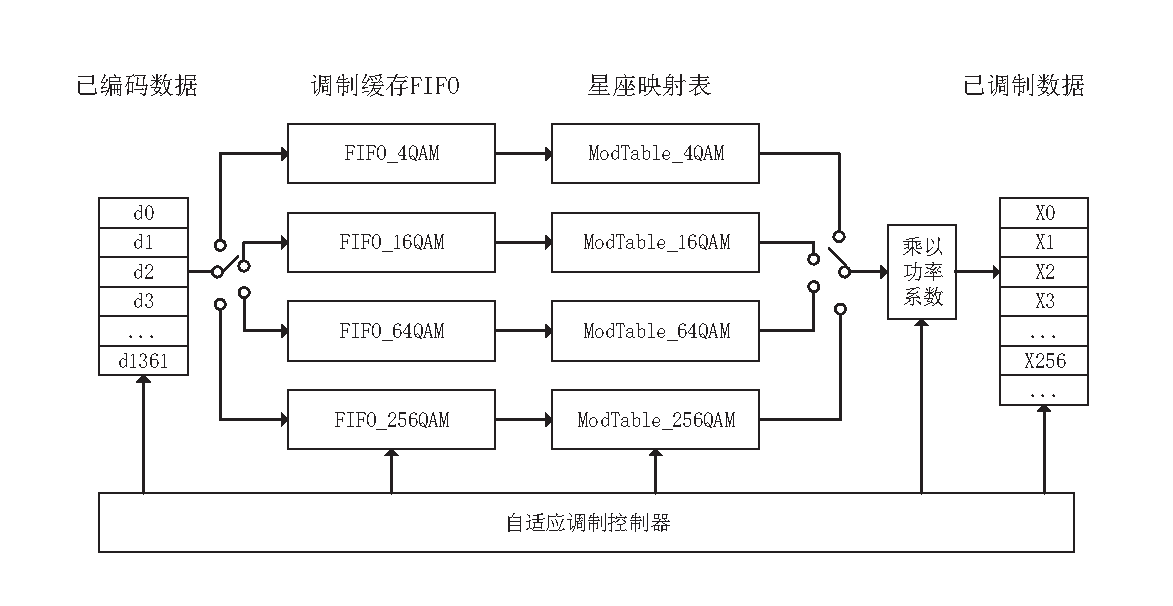
\includegraphics[width=0.9\textwidth]{figures/chapter-5/AdaptiveModulation.eps}
\caption{自适应调制模块示意图}
\label{fig:AdaptiveModulation}
\end{figure}
发射端的自适应调制模块设计如图\ref{fig:AdaptiveModulation}所示,已完成信道编码的数据放在一个位宽为8 bit的RAM中,现在要将这些数据分配到各个子载波上,本系统设计中我们的调制方式限定为4QAM、16QAM、64QAM和256QAM,而每种不同的调制每个符号能够携带的信息比特数也不同,每个M-QAM携带的比特数为$\log_2(M)$。因此先要把已编码的数据根据比特分配表放到不同的FIFO中去,因为FIFO的性质是FIFO的数据位宽要是输入输出的位宽的倍数,所以用于缓存FIFO的位宽及输入输出位宽如下表所示:
\begin{table}[ht]
    \caption{调制器FIFO参数设置}
    \label{tab:Signle Color Channel Estimation Paramters}
    \centering
    \begin{tabular}{llll}
        \toprule
        FIFO                & 数据位宽  &输入位宽  &输出位宽\\
        \midrule
		FIFO\_4QAM			& 8 bit		&8 bit    & 2 bit  \\
		FIFO\_16QAM			& 8 bit       &8 bit    & 4 bit  \\
		FIFO\_64QAM          & 24 bit       &24 bit    & 6 bit   \\
		FIFO\_64QAM			& 8 bit         &8 bit    & 8 bit  \\
        \bottomrule
    \end{tabular}
\end{table}
所以对于64QAM调制,缓存时需要先拼成24 bit输入,在以6 bit位宽读出。

数据缓存之后,使用查表法进行星座映射。具体是先把各阶QAM调制的已归一化星座点存到不同的ROM中,实部和虚部都按14 bit量化,然后按照各个子载波上的调制阶数,依次从各个FIFO中读出数据,并以此数据为地址,去读该调制下的星座图ROM,输出的数据就是归一化过的星座点,最后再根据功率分配表,乘上功率系数之后存到RAM缓存,同时要注意与之前固定调制不同,这里考虑的功率分配的因素,所以为了接收端简化起见,要在导频ZC序列上各个子载波也要乘以功率系数,这样接收端在解调的时候就不要再专门除以功率系数,会在单系数均衡中处理掉。整个自适应调制器由一个专门的控制器模块来进行时序控制和状态转换。

\subsection{信噪比估计与自适应参数计算}
\begin{figure}[htbp]
\centering
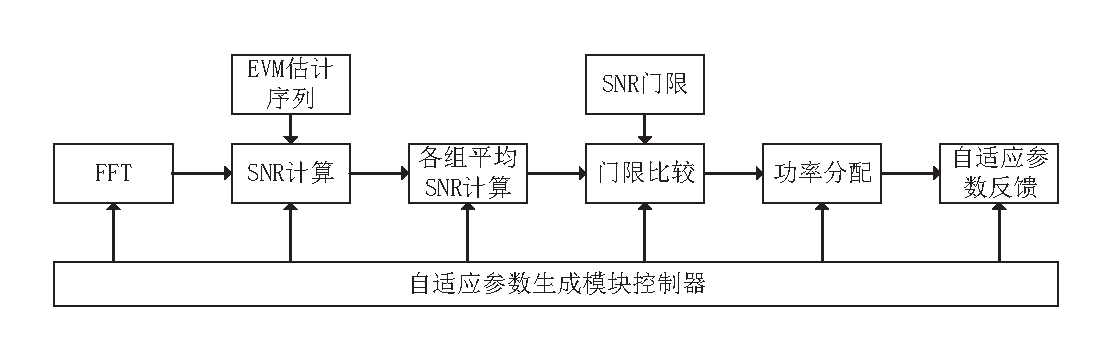
\includegraphics[width=0.9\textwidth]{figures/chapter-5/AdaptiveParameterGenerator.eps}
\caption{自适应参数生成模块示意图}
\label{fig:AdaptiveParameterGenerator}
\end{figure}
信噪比估计及自适应参数计算方案设计如图\ref{fig:AdaptiveParameterGenerator}所示,之前也提过,系统要传输专门的EVM序列来进行SNR估计,这样的帧成为EVM 帧,可以隔固定的时间发送一次,所以处理EVM帧其实就是求当前信道下的自适应参数。

EVM序列频域符号在接收端也是已知的,所以得到已经均衡过的时域符号之后,可以根据公式求得各个子载波上的SNR和噪声方差,每个OFDM符号都能得到一组SNR和噪声方差,可以通过几组值相加求平均的方法来提高估计精度。得到各个子载波上的SNR之后,根据设置的子载波总数和组数,求得每组子载波的平均SNR,然后利用Improved-SBLA 算法来进行比特和功率分配,为了简便起见,保证系统的鲁棒性,我们设置目标BER为$10^{-2}$,同时只按原算法进行初始分配,而不设置目标速率,这样就少了算法后来的循环累加或类减过程。在门限比较时,可以从高门限到低门限比较,当遇到SNR大于某个门限时,就取其对应的调制阶数。得到各个子载波组上分配的比特之后,使用公式求得各个子载波组的第一个子载波和最后一个子载波的功率。将此比特分配和功率分配按照一定的数据格式发送给发射端。
\subsection{自适应软解调模块}
\begin{figure}[htbp]
\centering
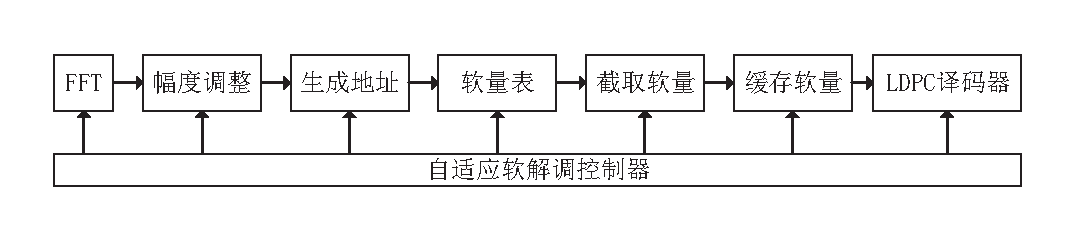
\includegraphics[width=0.9\textwidth]{figures/chapter-5/AdaptiveDemodulation.eps}
\caption{自适应软解调模块示意图}
\label{fig:AdaptiveDemodulation}
\end{figure}
当传输的是数据帧时,自适应软解调按图\ref{fig:AdaptiveDemodulation}所示方案进行软解调,其基本思路是查表法,并且只使用256QAM调制一张表,其他的三种低阶调制通过一些数据变换来时候这张表,按照软量计算理论,实部和虚部分开进行软量计算,并且使用的方法是一样的。下面来介绍具体过程。

经过了单系数均衡后的各个子载波上的频域符号先要进行幅度调制,即乘以其对应的调制阶数的归一化因子,恢复各个调制符号在原始星座图上的幅度,并且要根据调制阶数进行相应的饱和处理,将其限定在对应星座图的范围内,如256-QAM限定在(-16,16)的范围内,64-QAM限定在(-8,8)范围内。然后采用坐标平移的方法让低阶调制能够使用256QAM的软量表,需要对其坐标点搬移到最高阶调制星座图上的合适位置。首先读取当前子载波所用的调制阶数以进行判断,从最低的4QAM移动到16QAM 坐标值减2,16QAM移动到64QAM坐标值减4,以此类推,即$2^k$-QAM向高阶移一阶坐标值减$2^k$/2。因此,对于本设计中各种调制都要移动到256QAM上,256QAM 本身不用移动,64QAM 要减去8,16QAM减去12,4QAM减去14。这样处理完了之后的实部和虚部数据就可以去查软量表了。因为对应的软量是256QAM的,并且软量是按8 bit 量化的,所以从软量表输出的是 32($4\times 8$)bit软量,而低阶调制只是取其中的一部分,如4QAM实部和虚部各传输1 bit,所以取软量表输出最后的8 bit,依次类推就能得到所有的比特软量了。从前所述不难看出,各个OFDM子载波因为调制阶数的不同,所以生成比特软量的速率也不同,所以要把得到的软量按顺序缓存下来,再送入LDPC译码器。

\section{系统展示}
本课题设计的硬件平台如图\ref{fig:Demo}所示,左边的三台计算机用于产生发射信源,T\_Red、T\_Blue和T\_Green发出的数据分别通过多色LED 的红光、蓝光和绿光三个通道发送到接收端;右边三台计算机R\_Red、R\_Blue和R\_Green接收响应色光的数据并显示。

\begin{figure}[htbp]
\centering
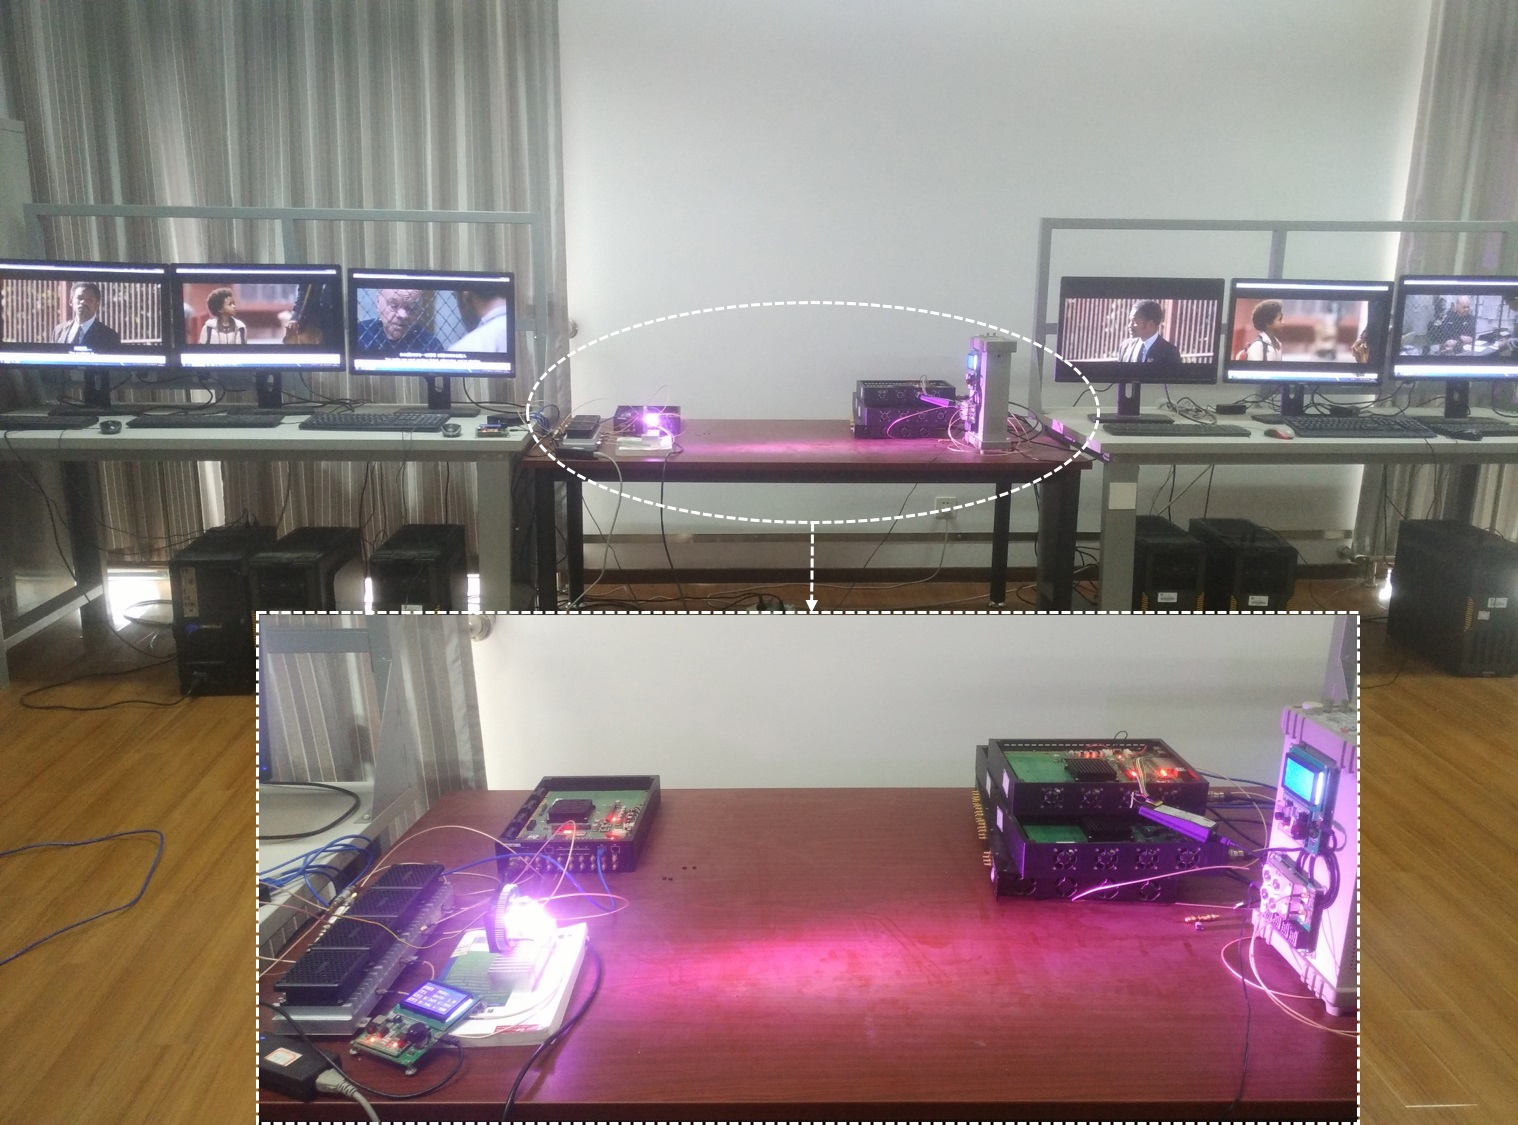
\includegraphics[width=0.9\textwidth]{figures/chapter-5/Demo.jpg}
\caption{硬件平台展示}
\label{fig:Demo}
\end{figure}




\section{本章小结}
本章在前面几章讲解可见光通信原理及其自适应传输理论的基础上,介绍了本课题对应的硬件平台。首先对整个硬件平台进行了概述,包括各种器件的参数及其选择依据,并且简述了发射端和接收端的基带处理处理过程;然后重点描述了基带处理中与自适应技术密切相关的调制器、自适应参数生成、软解调三个模块;最后展示了整个硬件平台实物图。
